% Source-faithful schematic draft: 2004 Chongqing Arts Q12, PDF p.1 (printed p.162).
% Source ID: src-8740ec31a416866bbb4486815be256dded62698124e78db56804308ae880dc2c
% Source SHA-256: e6d7fbbb3d22ed4e305929e1aa382abf4606838acacfa7c0b2e055313a891931
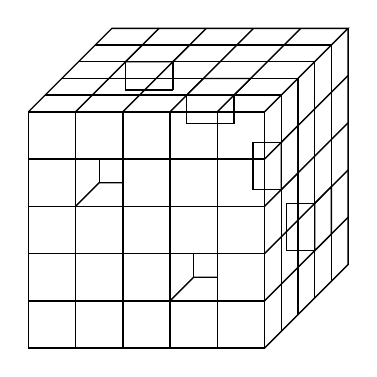
\begin{tikzpicture}[line width=0.5pt, scale=0.6, baseline=(current bounding box.center)]
  % Basis projection vector for depth (y-axis)
  \def\ux{0.3535}
  \def\uy{0.3535}

  % Front face grid (5x5)
  \draw (0,0) rectangle (5,5);
  \foreach \k in {1,2,3,4} {
    \draw (0,\k) -- (5,\k);
    \draw (\k,0) -- (\k,5);
  }

  % Top face grid (5x5)
  \draw (0,5) -- ({5*\ux}, {5+5*\uy}) -- ({5+5*\ux}, {5+5*\uy}) -- (5,5);
  \foreach \k in {1,2,3,4} {
    \draw (\k,5) -- ({\k+5*\ux}, {5+5*\uy});
    \draw ({\k*\ux}, {5+\k*\uy}) -- ({5+\k*\ux}, {5+\k*\uy});
  }

  % Right face grid (5x5)
  \draw (5,0) -- ({5+5*\ux}, {5*\uy}) -- ({5+5*\ux}, {5+5*\uy});
  \foreach \k in {1,2,3,4} {
    \draw (5,\k) -- ({5+5*\ux}, {\k+5*\uy});
    \draw ({5+\k*\ux}, {\k*\uy}) -- ({5+\k*\ux}, {5+\k*\uy});
  }

  % 1. Front face holes: fill white & draw frame & interior
  % Hole 1: col 2, row 4 ([1,2] x [3,4])
  \fill[white] (1.02, 3.02) rectangle (1.98, 3.98);
  \draw (1,3) rectangle (2,4);
  \draw (1,3) -- (1.5, 3.5) -- (2, 3.5);
  \draw (1.5, 3.5) -- (1.5, 4);

  % Hole 2: col 4, row 2 ([3,4] x [1,2])
  \fill[white] (3.02, 1.02) rectangle (3.98, 1.98);
  \draw (3,1) rectangle (4,2);
  \draw (3,1) -- (3.5, 1.5) -- (4, 1.5);
  \draw (3.5, 1.5) -- (3.5, 2);

  % 2. Top face holes: fill white parallelogram & interior
  % Hole 1 at col 2, depth 4: x in [1,2], y in [3,4]
  \fill[white] ({1+3*\ux+0.02}, {5+3*\uy+0.02}) -- ({2+3*\ux-0.02}, {5+3*\uy+0.02}) -- ({2+4*\ux-0.02}, {5+4*\uy-0.02}) -- ({1+4*\ux+0.02}, {5+4*\uy-0.02}) -- cycle;
  \draw ({1+3*\ux}, {5+3*\uy}) -- ({2+3*\ux}, {5+3*\uy}) -- ({2+4*\ux}, {5+4*\uy}) -- ({1+4*\ux}, {5+4*\uy}) -- cycle;
  \draw ({1+3*\ux}, {5+3*\uy}) -- ({1+3*\ux}, {4.4+3*\uy}) -- ({2+3*\ux}, {4.4+3*\uy});
  \draw ({2+3*\ux}, {5+3*\uy}) -- ({2+3*\ux}, {4.4+3*\uy});

  % Hole 2 at col 4, depth 2: x in [3,4], y in [1,2]
  \fill[white] ({3+1*\ux+0.02}, {5+1*\uy+0.02}) -- ({4+1*\ux-0.02}, {5+1*\uy+0.02}) -- ({4+2*\ux-0.02}, {5+2*\uy-0.02}) -- ({3+2*\ux+0.02}, {5+2*\uy-0.02}) -- cycle;
  \draw ({3+1*\ux}, {5+1*\uy}) -- ({4+1*\ux}, {5+1*\uy}) -- ({4+2*\ux}, {5+2*\uy}) -- ({3+2*\ux}, {5+2*\uy}) -- cycle;
  \draw ({3+1*\ux}, {5+1*\uy}) -- ({3+1*\ux}, {4.4+1*\uy}) -- ({4+1*\ux}, {4.4+1*\uy});
  \draw ({4+1*\ux}, {5+1*\uy}) -- ({4+1*\ux}, {4.4+1*\uy});

  % 3. Right face holes: fill white parallelogram & interior
  % Hole 1 at depth 2, row 4: y in [1,2], z in [3,4]
  \fill[white] ({5+1*\ux+0.02}, {3+1*\uy+0.02}) -- ({5+2*\ux-0.02}, {3+2*\uy-0.02}) -- ({5+2*\ux-0.02}, {4+2*\uy-0.02}) -- ({5+1*\ux+0.02}, {4+1*\uy-0.02}) -- cycle;
  \draw ({5+1*\ux}, {3+1*\uy}) -- ({5+2*\ux}, {3+2*\uy}) -- ({5+2*\ux}, {4+2*\uy}) -- ({5+1*\ux}, {4+1*\uy}) -- cycle;
  \draw ({5+1*\ux}, {3+1*\uy}) -- ({4.4+1*\ux}, {3+1*\uy}) -- ({4.4+1*\ux}, {4+1*\uy});
  \draw ({5+1*\ux}, {4+1*\uy}) -- ({4.4+1*\ux}, {4+1*\uy});

  % Hole 2 at depth 4, row 2: y in [3,4], z in [1,2]
  \fill[white] ({5+3*\ux+0.02}, {1+3*\uy+0.02}) -- ({5+4*\ux-0.02}, {1+4*\uy-0.02}) -- ({5+4*\ux-0.02}, {2+4*\uy-0.02}) -- ({5+3*\ux+0.02}, {2+3*\uy-0.02}) -- cycle;
  \draw ({5+3*\ux}, {1+3*\uy}) -- ({5+4*\ux}, {1+4*\uy}) -- ({5+4*\ux}, {2+4*\uy}) -- ({5+3*\ux}, {2+3*\uy}) -- cycle;
  \draw ({5+3*\ux}, {1+3*\uy}) -- ({4.4+3*\ux}, {1+3*\uy}) -- ({4.4+3*\ux}, {2+3*\uy});
  \draw ({5+3*\ux}, {2+3*\uy}) -- ({4.4+3*\ux}, {2+3*\uy});

\end{tikzpicture}
